\subsection{Testing Performed}
Due to the domain of this project and the technologies adopted, it was not as straightforward to 
test the raw performance of the system. As there is no performance metric or such that can be 
analysed and compares to other instances \cite{Samini2017}. 
\subsubsection{On-Site Testing}
Several test were performed on-site, where the locations were actually based, all in aims of exploring how the system handles different cases. 
This included normal usability and even edge cases such as using the panel where we know plane detection will struggle.
\\
The panel was tested on floors that had discernable planes features, and on others where there was a repeated pattern (a known struggle-point of plane detection).\\
% \begin{figure}[h]
%     \caption{some caption}
%     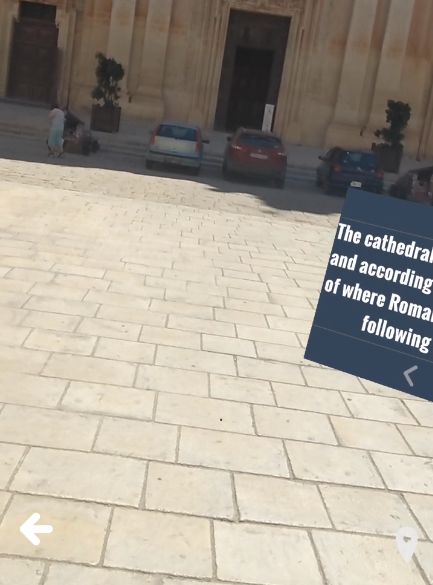
\includegraphics[width=8cm]{bad_floor_panel_glitch}
%     \end{figure}


% \begin{figure}[h]
%     \centering
%     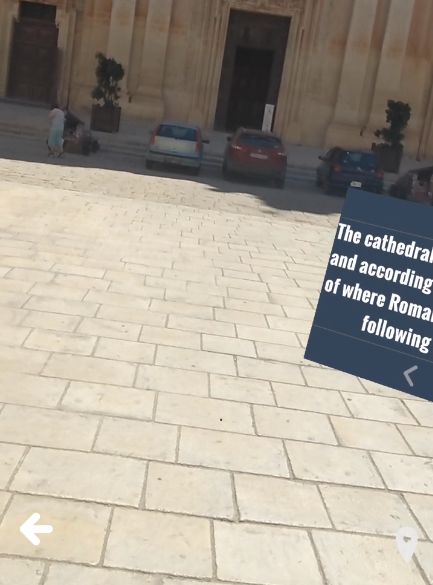
\includegraphics[width=.5\textwidth]{bad_floor_panel_glitch}
%     \caption{Panel Glitching due to repeated pattern}
%     \label{fig:bad_panel}
%     \end{figure}

%     \begin{figure}[h]
%         \centering
%         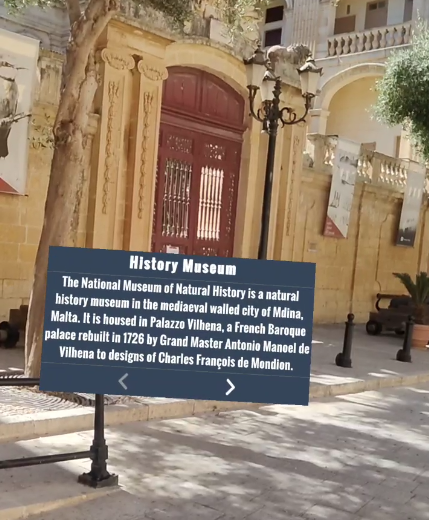
\includegraphics[width=.5\textwidth]{history_museum_text_panel}
%         \caption{Panel text}
%         \label{fig:panel_text}
%         \end{figure}

%         \begin{figure}[h]
%             \centering
%             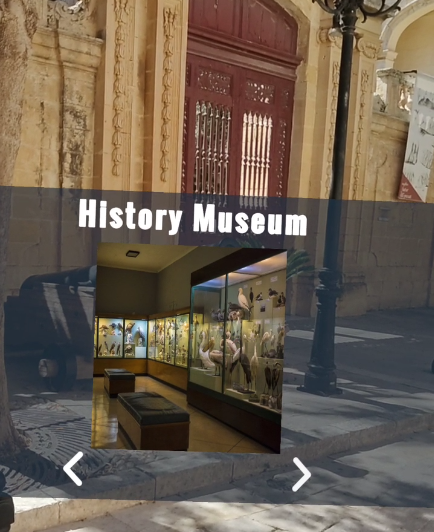
\includegraphics[width=.5\textwidth]{history_museum_image_panel1}
%             \caption{Panel img}
%             \label{fig:panel_img}
%             \end{figure}
\begin{figure}[!htb]
    \minipage{0.32\textwidth}
        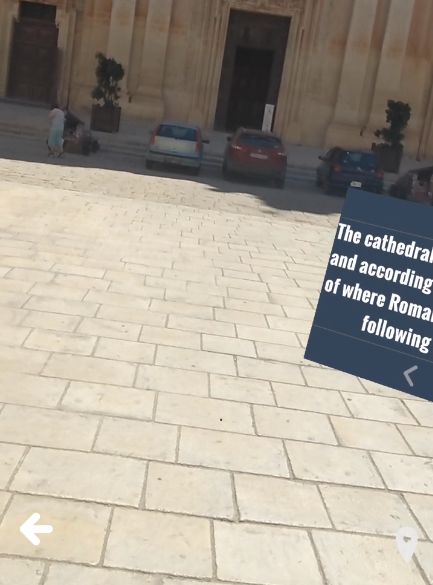
\includegraphics[width=\linewidth]{bad_floor_panel_glitch}
            \caption{Panel Glitching due to repeated pattern}
            \label{fig:bad_panel}
    \endminipage\hfill
    \minipage{0.32\textwidth}
        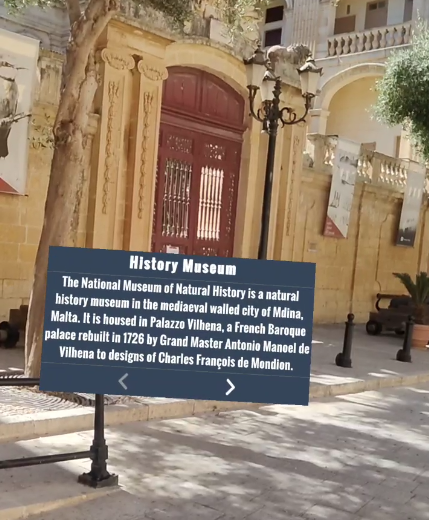
\includegraphics[width=\linewidth]{history_museum_text_panel}
        \caption{Stable Panel showing text}
        \label{fig:panel_text}
    \endminipage\hfill
    \minipage{0.32\textwidth}%
        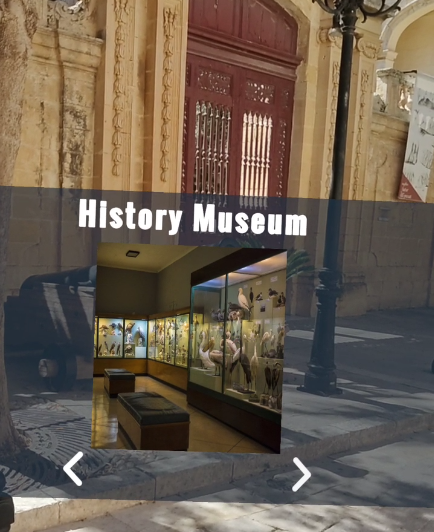
\includegraphics[width=\linewidth]{history_museum_image_panel1}
        \caption{Stable Panel showing image}
        \label{fig:panel_img}
    \endminipage
    \end{figure}         
Further testing is shown in the video, as it's the easiest way to show off the experience.\\
The application was also used with a subpar GPS connection (as some parts of Mdina do not have good coverage).\\
In order to test the  bearing accuracy, the north pole was temporarily added as a landmark, and a general comparison between the bearing shown and a compass was used.\\
Due to the centralised nature of the application, an internet connection needs to be maintained for most features to work, 
as all landmark information is obtained from the server.
\begin{figure}[!htb]
    \minipage{0.45\textwidth}
        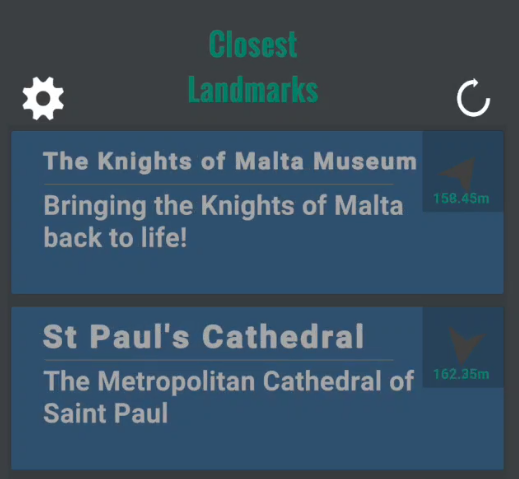
\includegraphics[width=\linewidth]{landmarks_menu}
            \caption{Explorable Landmark Entries}
            \label{fig:explor_lands}
    \endminipage\hfill
    \minipage{0.45\textwidth}
        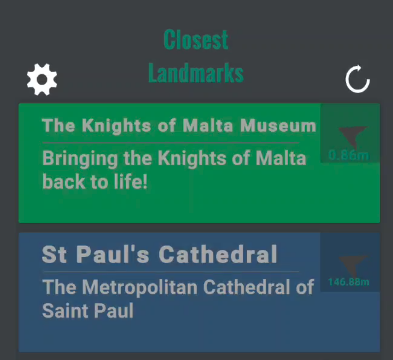
\includegraphics[width=\linewidth]{landmarks_menu_activated}
        \caption{Landmark Entry Activated}
        \label{fig:active_land}
    \endminipage
    \end{figure}    
\subsubsection{Augmented Images}
As augmented images were implemented some basic testing was also involved, where a simple image of the earth was detected, and overlayed with a 3D spinning globe. 
The image was recognized from different angles and light settings whilst tracking also was really responsive to even moving the image.
\begin{figure}[!htb]
    \minipage{0.32\textwidth}
        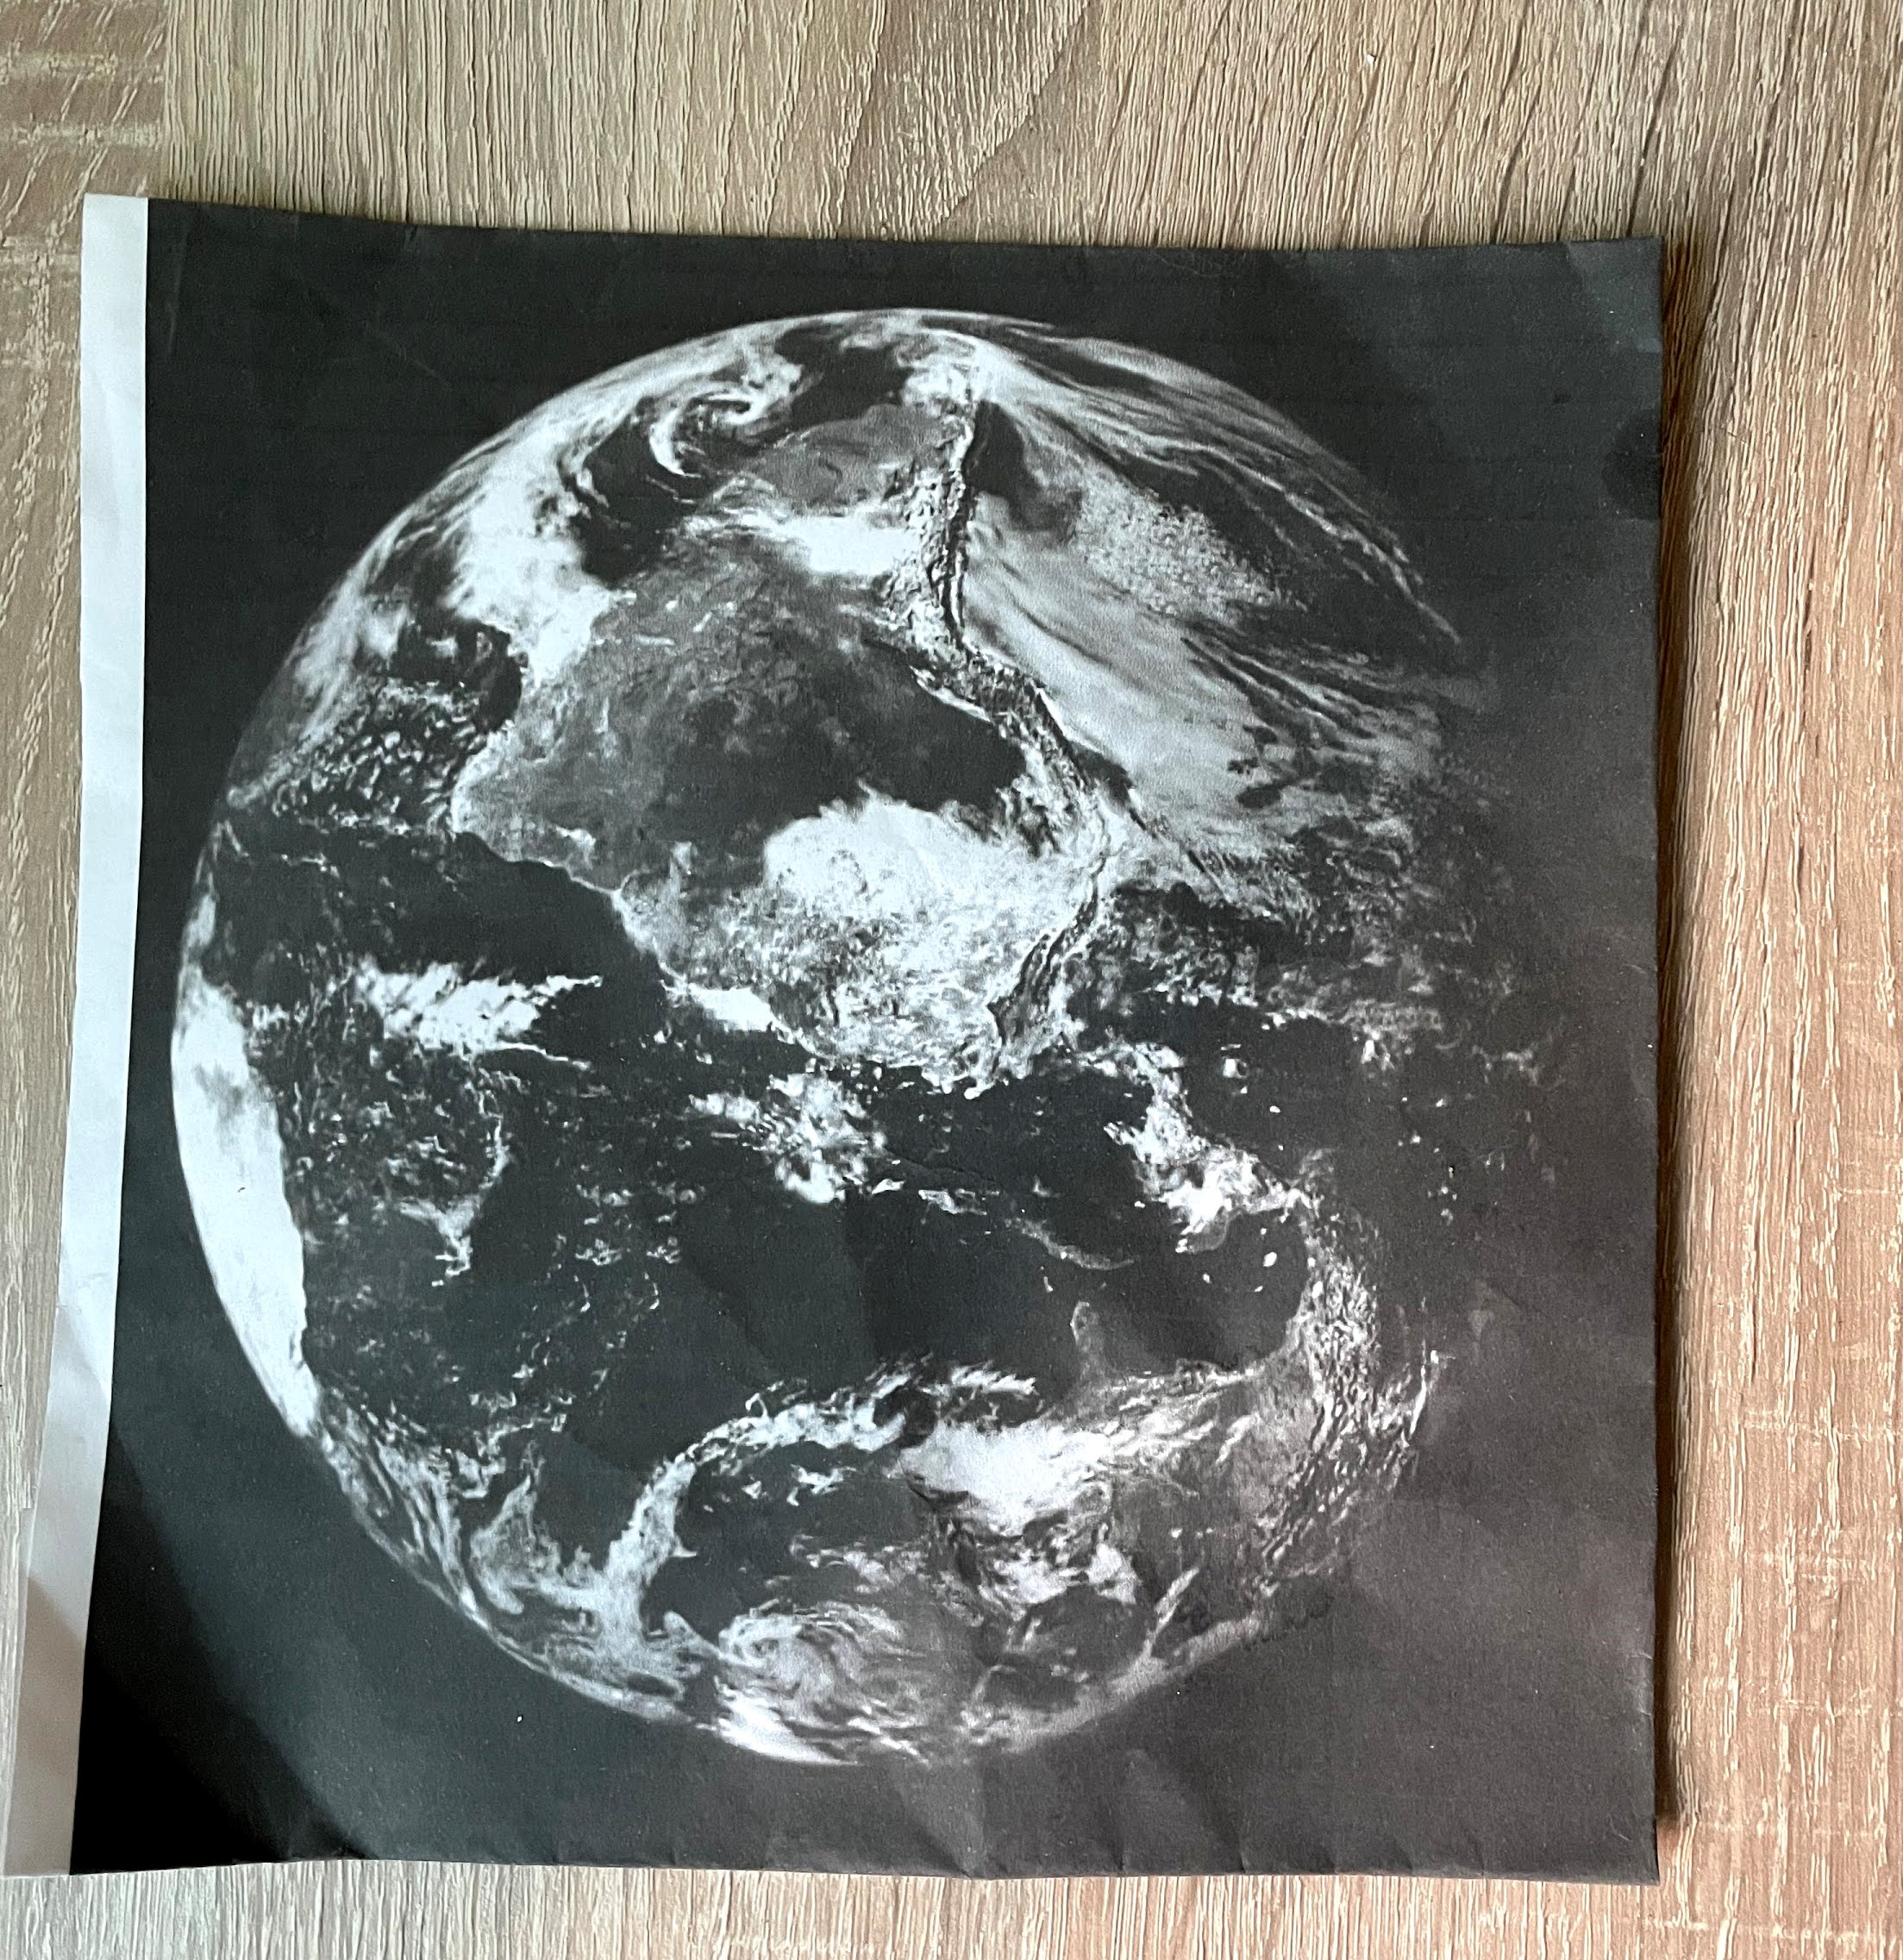
\includegraphics[width=\linewidth]{earth_og}
            \caption{Earth Image Key}
            \label{fig:earth_og}
    \endminipage\hfill
    \minipage{0.32\textwidth}
        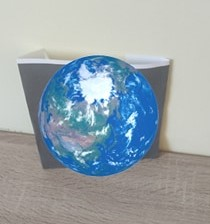
\includegraphics[width=\linewidth]{earth_ov}
        \caption{3D sphere overlayed}
        \label{fig:earth_ov}
    \endminipage
    \end{figure}
\subsection{Test Analysis}
\subsubsection{Landmark Menu}
The solution as an application was very stable in general, since unity was used, any changes can be done directly through the unity editor, and the benefits of being a 
unity-based applicaition are retained. The aim to provide some sense of direction to the user was also satisifed, as when the GPS connection was established, distance 
and bearing data was accurate. When the GPS connection was unstable, the bearing direction and distance was a little off, yet immediately normalized when conenction was restored. 
\subsubsection{AR Mode}
In general, when dsicernable plane features are present, the panel stays fixed in-place as intended.
However, plane detection by design, struggles when there are no close discernable attributes (the floor has a regular pattern for example), which the tests 
have also shown to affect the stability of the position of the panel.
\subsubsection{Server Communication}
Through using the application, the server was also being tested. The solution developed was very responsive, and provided very quick and usable results. 
Distance calculation and geofeincing also worked punctually, and the device's locations were updated in realtime.\\
As expandability was also in mind, it is really easy to add,remove and change landmarks, as a simple json file is provided, where every bit of details can be changed.

The few test perofrmed show that the technologies used are very applicable to the aims and objectives. The strengths of the application match up with the strengths of the domain, 
providing a deep sense of immersion and informative. The weknesses of the application are also in sync with the limitations of the domain. Particulary, the systems suffers where a stable 
plane is not detected and a plane with lower certainty has to be used, which may cause the information panel to shift positions unexpectedly. 

\subsection{Potential Testing}
Three key points mentioned in \cite{Samini2017} have great potential in giving a more formal understanding of the performance of such systems. 
\subsubsection{Independant Variables}
The variation of independent variables can be used as a performance metric and help analyse the experience of the user, these variables include things that are not 
varied by the user during the test. Examples of such variables include the device size and the field of view of a device's 
camera.\\
\subsubsection{Dependant Variables}
These variables give a robust metric of how the users react to the 
application presented, such as the number of attempts taken to carry out an action.
Yet this is very application-specific and does not allow for comparison between other systems, as 
tasks in an application usually are specific to it.

\subsubsection{Questionnaires}
Questionnaires were mentioned as another performance metric, which allows a subjective metric. 
In applications such as the tourism domain, this is of utmost importance, as it follows that 
from the user-centric nature, the ultimate goal is the users' experience.  

% \subsection{Future Works}
% The system was developed with expandability in mind, and thus, it is really easy to adapt the system into different uses cases.
\subsection{Possible Improvements}
\subsubsection{Augmented Images}
Ideally, augmented imaging is implemented as another landmark type, as it would allow for a wider range of applications and immersion.
This application would also be applcable in places such as inside museums where for example it would enchance a painting, or have some animation overlayed on it.

Another possible improvment is to give better direction towards landmarks, the current application simply gives baring direction and straight line distance between points,
 without any consideration for the streets/obstacles.
\subsection{Future Work}
During development, it was made sure to keep the system as open as possible. Through the 
centralised API, unity engine and other technologies used, the system is meant to be dynamic and 
expandable.\\
With minimal effort, it can be easily be adapted to different uses such as an AR game, 
using google APIs for international standardized locations or even showing 3D models in AR mode. 

